\documentclass[12pt]{article}
%%---------------------------------------------------------------------
% packages
% geometry
\usepackage{geometry}
% font
\usepackage{fontspec}
\defaultfontfeatures{Mapping=tex-text}  %%如果没有它,会有一些 tex 特殊字符无法正常使用,比如连字符。
\usepackage{xunicode,xltxtra}
\usepackage[BoldFont,SlantFont,CJKnumber,CJKchecksingle]{xeCJK}  % \CJKnumber{12345}: 一万二千三百四十五
\usepackage{CJKfntef}  %%实现对汉字加点、下划线等。
\usepackage{pifont}  % \ding{}
% math
\usepackage{amsmath,amsfonts,amssymb}
% color
\usepackage{color}
\usepackage{xcolor}
\definecolor{EYE}{RGB}{199,237,204}
\definecolor{FLY}{RGB}{128,0,128}
\definecolor{ZHY}{RGB}{139,0,255}
% graphics
\usepackage[americaninductors,europeanresistors]{circuitikz}
\usepackage{tikz}
\usetikzlibrary{positioning,arrows,shadows,shapes,calc,mindmap,trees,backgrounds}  % placements=positioning
\usepackage{graphicx}  % \includegraphics[]{}
\usepackage{subfigure}  %%图形或表格并排排列
% table
\usepackage{colortbl,dcolumn}  %% 彩色表格
\usepackage{multirow}
\usepackage{multicol}
\usepackage{booktabs}
% code
\usepackage{fancyvrb}
\usepackage{listings}
% title
\usepackage{titlesec}
% head/foot
\usepackage{fancyhdr}
% ref
\usepackage{hyperref}
% pagecolor
\usepackage[pagecolor={EYE}]{pagecolor}
% tightly-packed lists
\usepackage{mdwlist}

\usepackage{styles/iplouccfg}
\usepackage{styles/zhfontcfg}
\usepackage{styles/iplouclistings}

%%---------------------------------------------------------------------
% settings
% geometry
\geometry{left=2cm,right=1cm,top=2cm,bottom=2cm}  %设置 上、左、下、右 页边距
\linespread{1.5} %行间距
% font
\setCJKmainfont{Adobe Kaiti Std}
%\setmainfont[BoldFont=Adobe Garamond Pro Bold]{Apple Garamond}  % 英文字体
%\setmainfont[BoldFont=Adobe Garamond Pro Bold,SmallCapsFont=Apple Garamond,SmallCapsFeatures={Scale=0.7}]{Apple Garamond}  %%苹果字体没有SmallCaps
\setCJKmonofont{Adobe Fangsong Std}
% graphics
\graphicspath{{figures/}}
\tikzset{
    % Define standard arrow tip
    >=stealth',
    % Define style for boxes
    punkt/.style={
           rectangle,
           rounded corners,
           draw=black, very thick,
           text width=6.5em,
           minimum height=2em,
           text centered},
    % Define arrow style
    pil/.style={
           ->,
           thick,
           shorten <=2pt,
           shorten >=2pt,},
    % Define style for FlyZhyBall
    FlyZhyBall/.style={
      circle,
      minimum size=6mm,
      inner sep=0.5pt,
      ball color=red!50!blue,
      text=white,},
    % Define style for FlyZhyRectangle
    FlyZhyRectangle/.style={
      rectangle,
      rounded corners,
      minimum size=6mm,
      ball color=red!50!blue,
      text=white,},
    % Define style for zhyfly
    zhyfly/.style={
      rectangle,
      rounded corners,
      minimum size=6mm,
      ball color=red!25!blue,
      text=white,},
    % Define style for new rectangle
    nrectangle/.style={
      rectangle,
      draw=#1!50,
      fill=#1!20,
      minimum size=5mm,
      inner sep=0.1pt,}
}
\ctikzset{
  bipoles/length=.8cm
}
% code
\lstnewenvironment{VHDLcode}[1][]{%
  \lstset{
    basicstyle=\footnotesize\ttfamily\color{black},%
    columns=flexible,%
    framexleftmargin=.7mm,frame=shadowbox,%
    rulesepcolor=\color{blue},%
%    frame=single,%
    backgroundcolor=\color{yellow!20},%
    xleftmargin=1.2\fboxsep,%
    xrightmargin=.7\fboxsep,%
    numbers=left,numberstyle=\tiny\color{blue},%
    numberblanklines=false,numbersep=7pt,%
    language=VHDL%
    }\lstset{#1}}{}
\lstnewenvironment{VHDLmiddle}[1][]{%
  \lstset{
    basicstyle=\scriptsize\ttfamily\color{black},%
    columns=flexible,%
    framexleftmargin=.7mm,frame=shadowbox,%
    rulesepcolor=\color{blue},%
%    frame=single,%
    backgroundcolor=\color{yellow!20},%
    xleftmargin=1.2\fboxsep,%
    xrightmargin=.7\fboxsep,%
    numbers=left,numberstyle=\tiny\color{blue},%
    numberblanklines=false,numbersep=7pt,%
    language=VHDL%
    }\lstset{#1}}{}
\lstnewenvironment{VHDLsmall}[1][]{%
  \lstset{
    basicstyle=\tiny\ttfamily\color{black},%
    columns=flexible,%
    framexleftmargin=.7mm,frame=shadowbox,%
    rulesepcolor=\color{blue},%
%    frame=single,%
    backgroundcolor=\color{yellow!20},%
    xleftmargin=1.2\fboxsep,%
    xrightmargin=.7\fboxsep,%
    numbers=left,numberstyle=\tiny\color{blue},%
    numberblanklines=false,numbersep=7pt,%
    language=VHDL%
    }\lstset{#1}}{}
% pdf
\hypersetup{pdfpagemode=FullScreen,%
            pdfauthor={Haiyong Zheng},%
            pdftitle={Title},%
            CJKbookmarks=true,%
            bookmarksnumbered=true,%
            bookmarksopen=false,%
            plainpages=false,%
            colorlinks=true,%
            citecolor=green,%
            filecolor=magenta,%
            linkcolor=cyan,%red(default)
            urlcolor=cyan}
% section
%http://tex.stackexchange.com/questions/34288/how-to-place-a-shaded-box-around-a-section-label-and-name
\newcommand\titlebar{%
\tikz[baseline,trim left=3.1cm,trim right=3cm] {
    \fill [cyan!25] (2.5cm,-1ex) rectangle (\textwidth+3.1cm,2.5ex);
    \node [
        fill=cyan!60!white,
        anchor= base east,
        rounded rectangle,
        minimum height=3.5ex] at (3cm,0) {
        \textbf{\thesection.}
    };
}%
}
\titleformat{\section}{\Large\bf\color{blue}}{\titlebar}{0.1cm}{}
% head/foot
\setlength{\headheight}{15pt}
\pagestyle{fancy}
\fancyhf{}
%\lhead{\color{black!50!green}2014年秋季学期}
\chead{\color{black!50!green}Feature Contrasts\&Priors}
%\rhead{\color{black!50!green}通信电子电路}
\lfoot{\color{blue!50!green}朱亚菲}
\cfoot{\color{blue!50!green}\href{http://vision.ouc.edu.cn/~zhenghaiyong}{CVBIOUC}}
\rfoot{\color{blue!50!green}$\cdot$\ \thepage\ $\cdot$}
\renewcommand{\headrulewidth}{0.4pt}
\renewcommand{\footrulewidth}{0.4pt}


%%---------------------------------------------------------------------
\begin{document}
%%---------------------------------------------------------------------
%%---------------------------------------------------------------------
% \titlepage
\title{\vspace{-2em}显著性检测领域之feature contrasts和priors\vspace{-0.7em}}
\author{朱亚菲}
\date{\vspace{-0.7em}2015年1月\vspace{-0.7em}}
%%---------------------------------------------------------------------
\maketitle\thispagestyle{fancy}
%%---------------------------------------------------------------------
\maketitle
\tableofcontents 


\section{引言}

\subsection{显著性检测}

人类视觉系统对复杂场景具有强适应性,神经生理和心理学研究表明人眼面临复杂场景时,会迅速将注意力集中在少数重要区域,并利用有限的处理能力对其优先处理。图像显著性检测的目的是在图像中快速有效地找到重要并且信息量大的区域~\cite{li2013contextual}。目前在图像重定向、图像分类、图像分割等领域都有广泛的应用。

目前大多数显著性检测方法都是基于自底向上的计算框架。归纳起来通常分为三步:1. 特征提取,提取多种视觉特征,例如亮度、颜色、纹理等。2. 求像素或区域间的对比度。3. 求显著图

\subsection{features}

图像特征提取是图像分析与图像识别的前提,它是将高维的图像数据进行简化表达最有效的方式,从一幅图像的$M \times N \times3$的数据矩阵中,我们看不出任何信息,所以我们必须根据这些数据提取出图像中的关键信息,一些基本元件以及它们的关系。

图像特征可分为全局特征和局部特征\footnote{更多局部特征见\url{http://www.sigvc.org/bbs/thread-165-1-1.html}}。其最大的区别是特征提取的空间范围不同。全局特征是从整个图像中提取的特征,而局部特征是从图像区域中提取的特征。全局特征容易受到环境的干扰,光照、旋转、噪声等不利因素都会影响全局特征。相比而言,局部特征点,往往对应着图像中的一些线条交叉、明暗变化的结构中,受到的干扰也少。

总的来说,全局特征是对图像内容的高度抽象的概括。如果用户对整个图像的整体感兴趣,而不是对前景本身感兴趣的话,用全局特征来描述图像是比较合适的。但是无法分辨出前景和背景却是全局特征本身就有的劣势,特别是在关注的对象受到遮挡等影响的时候,全局特征很有可能就被破坏掉了。

在显著性检测中,由于关注的是显著目标,并且是在同一幅图像中进行中央-周围/局部/全局对比,而不是在图像间进行比较,因此用到的应该都是局部特征。显著性检测领域所说的局部和全局方法是指对某一像素或区域,在计算其对比度时是与周围相比还是与图像中所有其它像素或区域相比。

英国Oxford大学的Andrea Valida,他是VLFeat(Vision Lab Features Library)的发起者和主要作者。VLFeat官方主页:\url{vlfeat.org}。它一个实现了计算机视觉领域诸多算法的开源库,包括SIFT,HOG等等。底层代码用C语言实现,并提供了MATLAB接口。支持Windows,Mac OS X和Linux。VLFeat目前正在逐渐实现其他常用的特征描述子。和OpenCV相比,VLFeat是一个轻量级的库,主要实现了在特征提取和聚类方面的高效算法,可以用在图像检索和物体识别领域中。

图像特征又可以分为低层次特征和高层次特征~\cite{nixon2012feature}。其中低层次特征是不需要任何形状信息(空间关系的信息)就可以从图像中自动提取的基本特征。高层次特征提取关心的是在图像中找出形状。例如,要自动识别人脸,一种方法是提取组成部分特征。也就是说,需要提取眼睛、耳朵和鼻子这些主要的脸部特征。这些特征可以利用它们的形状找到:眼睛的白色部分是椭圆形的;嘴巴可以看做是两条直线,眉毛也一样。形状提取意味着找出它们的位置、朝向和尺寸。所有低层次方法都可以应用于高层次特征提取,从而在图像中找到形状。(这里将特征分为低层次特征和高层次特征是是从广义还是狭义的角度我还没有搞清楚)

\subsection{feature contrasts}

对于一幅图像,人们会更加关注与周围物体的对比度差异大的区域。

\subsection{color space}

一般显著性检测方法中都会用到颜色特征。颜色通常用三个(也可以更多或更少)相对独立的属性来描述,三个独立变量综合作用,自然就构成一个空间坐标,这就是颜色空间。而颜色可以由不同的角度,用不同属性加以描述,就产生了不同的颜色空间。但被描述的颜色对象本身是客观的,不同颜色空间只是从不同的角度去衡量同一个对象。除了RGB颜色空间,另外两个常用的颜色空间就是CIELab和HSV颜色空间。

颜色空间按照基本结构可以分两大类:基色颜色空间和色、亮分离颜色空间。前者的典型是RGB,还包括CMY、CMYK、CIE XYZ等;后者包括YCC/YUV、Lab,以及一批“色相类颜色空间”。CIE XYZ是定义一切颜色空间的基准,很奇妙的是,它即属于基色颜色空间,也属于色、亮分离颜色空间,是贯穿两者的枢纽。色、亮分离颜色空间中的子类型”色相类颜色空间“,是把颜色分成一个表亮属性和两个表色属性,其中有一个表色属性是色相,而色相以外的两个属性可以选用不同的变量来定义,色相的概念不变,因此就构成一族共同使用色相属性,另加表亮属性和表色属性各一个组成的颜色空间,它们是颜色空间中的一个家族,暂且统称为HSB颜色空间。

\subsubsection{RGB颜色空间}

RGB颜色空间是常用的表示彩色图像的一种颜色空间,它是以红、绿、蓝三种颜色为基础,亦称为“三原色”。所谓的“原色”是一种生物学概念,是根据人眼对光线感知的生理作用来定义的。每一种颜色按亮度进行分类,分成256个等级。不同比例的红、绿、蓝叠加,能产生丰富的颜色。例如,等比例的三原色进行相加可以产生白色,红色与绿色相加产生黄色。可见,RGB空间属于“叠加型”原色系统,因此把RGB颜色空间作为最基础的颜色空间,通过对RGB的非线性或线性变换可以获得其它的颜色空间。

RGB颜色空间最常用的用途就是显示器系统,彩色阴极射线管、彩色光栅图形的显示器都使用R、G、B数值来驱动R、G、B电子枪发射电子,并分别激发荧光屏上的R、G、B三种颜色的荧光粉发出不同亮度的光线,并通过相加混合产生各种颜色;扫描仪也是通过吸收原稿经反射或透射而发送来的光线中的R、G、B成分,并用它来表示原稿的颜色。RGB色彩空间称为与设备相关的色彩空间,因为不同的扫描仪扫描同一幅图像,会得到不同色彩的图像数据;不同型号的显示器显示同一幅图像,也会有不同的色彩显示结果。

\subsubsection{YUV颜色空间}

在现代彩色电视系统中,通常采用三管彩色摄像机或彩色CCD(点耦合器件)摄像机,它把摄得的彩色图像信号经分色分别放大校正得到RGB,再经过矩阵变换电路得到亮度信号Y和两个色差信号$R-Y$、$B-Y$,最后发送端将亮度和色差三个信号分别进行编码,用同一信道发送出去。这就是我们常用的YUV色彩空间。采用YUV色彩空间的重要性是它的亮度信号Y和色度信号$U$、$V$是分离的。如果只有Y信号分量而没有$U$、$V$分量,那么这样表示的图就是黑白灰度图。彩色电视采用YUV空间正是为了用亮度信号Y解决彩色电视机与黑白电视机的兼容问题,使黑白电视机也能接收彩色信号。根据美国国家电视制式委员会,NTSC制式的标准,当白光的 亮度用Y来表示时,它和红、绿、蓝三色光的关系可用如下式的方程描述:$Y=0.3R+0.59G+0.11B$,这就是常用的亮度公式。色差$U$、$V$是由$B-Y$、$R-Y$按不同比例压缩而成的。如果要由YUV空间转化成RGB空间,只要进行 相反的逆运算即可。

\subsubsection{CIEXYZ颜色空间}

国际照明委员会(CIE)在进行了大量正常人视觉测量和统计的基础上,与1931年建立了“标准色度观察者”,从而奠定了现代CIE标准色度学的定量基础。在色彩管理中,选择与设备无关的颜色空间是十分重要的,与设备无关的颜色空间由国际照明委员会(CIE)制定,包括CIEXYZ和CIELAB两个标准。它们包含了人眼所能辨别的全部颜色。

\subsubsection{CIELUV颜色空间}

论文~\cite{ma2003contrast}中用到。

LUV色彩空间全称CIE 1976(L*,u*,v*)(也作CIELUV)色彩空间,L*表示物体亮度,u*和v*是色度。于1976年由国际照明委员会(International commission on Illumination)提出,由CIE XYZ空间经简单变换得到,具视觉统一性。类似的色彩空间有CIELAB。对于一般的图像,u*和v*的取值范围为-100到+100,亮度为0到100。

\subsubsection{CIELAB颜色空间}

Lab模式是由国际照明委员会(CIE)于1976年公布的一种色彩模式。它既不依赖光线,也不依赖于颜料,是CIE组织确定的一个理论上包括了人眼可以看见的所有色彩的色彩模式。CIELab颜色模型基于人对颜色的感觉,是一种接近人类视觉的颜色系统。Lab中的数值描述正常视力的人能够看到的所有颜色。因为Lab描述的是颜色的显示方式,而不是设备(如显示器、桌面打印机或数码相机)生成颜色所需的特定色料的数量,所以Lab被视为与设备无关的颜色模型。CIELab颜色空间是CIE XYZ颜色空间的一种数学变换的结果。

CIELAB系统使用的坐标叫做对色坐标(opponent color coordinate),使用对色坐标的想法来自这样的概念:颜色不能同时是红和绿,或者同时是黄和蓝,但颜色可以被认为是红和黄、红和蓝、绿和黄以及绿和蓝的组合。CIELAB使用L, a和b坐标轴定义CIE颜色空间。其中,L值代表光亮度,其值从0(黑色)~100(白色)。a和b代表色度坐标,其中a代表红-绿轴,b代表黄-蓝轴,取值范围是$[127, -128]$,如图~\ref{fig: Lab}。
\begin{figure}[!ht]
\centering
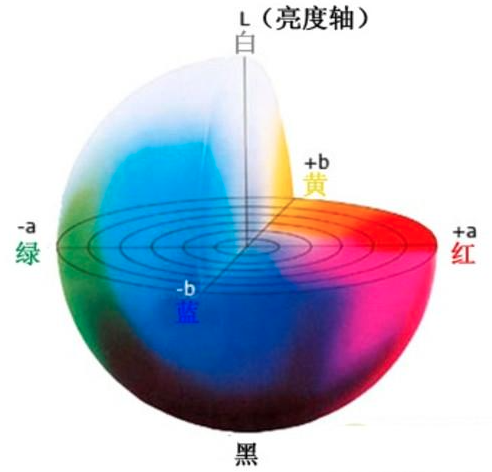
\includegraphics[width=0.3\textwidth]{Lab.png}
\caption{Lab颜色模型}
\label{fig: Lab}
\end{figure} 

matlab中由RGB空间转换到Lab空间的函数如下:
\lstinputlisting{rgb2lab.m} %用的CB方法中的

\subsubsection{HSV颜色模型}

HSV(Hue, Saturation, Value)是根据颜色的直观特性由A. R. Smith在1978年创建的一种颜色空间,也称六角椎体模型(Hexcone Model)。

HSV颜色模式是除了RGB颜色模式之外的另一种流行的颜色模式,RGB被广泛运用于计算机中,而HSV则用在电视显示方面。它更符合人们对颜色的描述(什么颜色(H),深浅度如何(S),亮度如何(V))。其实在电视机上菜单中的饱和度就是S,亮度就是V。

如图~\ref{fig: HSV},色调(H)用与水平轴之间的角度来表示,范围从0度到360度。六边形的顶点以60度为间隔。黄色位于60度处,绿色在120度处而青色在150度处,与红色相对。相补的颜色互成180度。

饱和度(S)从0到1变化。在此模型中它表示成所选色彩的纯度与该色彩的最大纯度($S=1$)的比率。当$S=0,5$时所选色彩的纯度为四分之一。当S=0 时,只有灰度。

亮度值(V)从六边形顶点的 0 变化到顶部的 1,顶点表示白色。在六边形顶部的颜色强度最大。当$ V=1$,$S=1$时,有纯色彩。白色是$V=1$且$S=0$的点。

\begin{figure}[!ht]
\centering
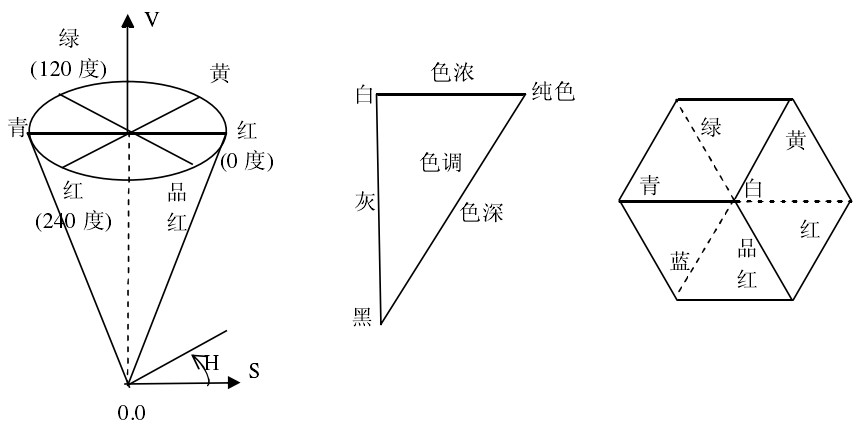
\includegraphics[width=0.6\textwidth]{HSV.jpg}
\caption{HSV颜色模型}
\label{fig: HSV}
\end{figure} 

matlab自带的rgb2hsv函数如下:
\lstinputlisting{rgb2hsv.m} 

总结:可以看到YUV/YIQ颜色空间是由RGB空间线性变换而来,而CIELab和HSV颜色空间则是由RGB空间非线性变换而来~\cite{kim2014salient}。

\section{基于像素点的feature contrasts}

\subsection{亮度}

Itti1998模型~\cite{itti1998model}中用到。亮度信息是最基本的视觉信息,它直接由视网膜的视杆细胞产生,是最基本的视觉信息,视觉系统中的其他信息很多也是由亮度而来。而从计算的角度考虑,亮度特征也足够用于多数图像处理任务,比如分割、识别,同时计算量远小于彩色特征。一些特殊成像方法得到的图像没有颜色信息,直接利用获取的亮度信息。

设r,g,b为输入图像的红色、绿色、蓝色通道,则Itti原始模型中亮度特征可以简单的计算出来:
\begin{align}
I = \frac{r+g+b}{3}
\end{align}

\subsection{颜色}

Itti1998模型~\cite{itti1998model}中用到。颜色信息由视网膜的三种视锥细胞分别产生,而在初级视觉皮层中的颜色柱进行重新组合。颜色柱中的神经细胞对颜色的选择呈现双拮抗性质,即一种颜色使得细胞产生兴奋,而另一种颜色使得能够抑制该细胞的兴奋。在人类视觉皮层中存在四种拮抗颜色对,分别是红-绿、绿-红、蓝-黄、黄-蓝。

首先为了去除颜色与亮度之间的耦合关系,用之前计算的亮度值对进行规一化处理。又因为视锥细胞只能在明亮的光线下感受颜色,所以只对亮度大于 图像中最大亮度10\%的区域进行规一化,而其他区域的均置为0。

数字图像一般只有红、绿、蓝三个颜色通道,为了得到黄色通道,Itti根据归一化后的,使用下面的公式计算广义上的红、绿、蓝、黄四个通道:
\begin{align}
R = r-\frac{g+b}{2}\\
G = r-\frac{r+b}{2}\\
B = r-\frac{r+g}{2}
\end{align}
接下来利用这四个通道计算红-绿、蓝-黄颜色对。Itti模型巧妙地利用绝对值,表示了两个相反的颜色对中兴奋的那一种。因此红-绿与绿-红颜色对可以用一个公式表示:
\begin{align}
RG = |R-G|\\
BY = |B-Y|
\end{align}

\subsection{方向}

Itti1998模型~\cite{itti1998model}中用到。初级视觉皮层细胞对特定方向的刺激有强烈反应。Dennis Gabor经过研究发现,二维 Gabor 滤波器非常适合表示这种反应。二维 Gabor滤波器是一种用于检测边缘的线性滤波器,由高斯核函数与一个余弦函数调制得到:
\begin{align}
g(x, y; \lambda, \theta, \psi, \delta, \gamma) = exp\left(-\frac{x'^2+\gamma^2y'^2}{2\delta^2}\right)sin(\frac{2\pi x'}{\lambda}+\psi)
\end{align}
其中$x'=xcos\theta+ysin\theta$,$y'=-xsin\theta+ycos\theta$。公式中$\lambda$表示余弦函数的波长,$\theta$表示Gabor滤波器的方向,$\psi$表示相位,$\gamma$表示空间长宽比,$\delta$表示高斯包络的标准差。

由于初级视觉皮层中有几千万个细胞,无法用模型将它们全部表示出来,Itti对这种生理结构进行了适当的简化。通过比较生理实验结果与模型的结果,固定次要变量,设置$ λ = 7$,$\psi= 0$,$\gamma = 1$,$\delta = 2.333$。而主要的变量是$\theta$,对 应着 Gabor滤波器的方向,Itti将连续的方向离散化,选择了4个最有代表性 的方向:$0^{\circ}$,$45^{\circ}$,$90^{\circ}$,$135^{\circ}$,这样就构造出4个Gabor滤波器,分别对输入图像滤波,得到 4 个方向特征图,记作$O(\theta)$,其中$\theta=0^{\circ}$,$45^{\circ}$,$90^{\circ}$,$135^{\circ}$。

\subsection{SIFT特征}

SIFT特征(Scale-invariant transform,尺度不变特征变换)由David Lowe在1999年~\cite{lowe1999object}所发表,2004年~\cite{lowe2004distinctive}完善总结。它是一种计算机视觉的算法,用来侦测与描述图像中的局部性特征,它在空间尺度中寻找极值点,并提取出其位置、尺度、旋转不变量。SIFT算法提取的特征点具有尺度不变性,也就是说,同一物体在图像上不论尺度大小,都能根据SIFT算法提取到相同的特征点。

简单来说,SIFT算法就是用不同尺度(标准差)的高斯函数对图像进行平滑,然后比较平滑后图像的差别,差别大的像素就是特征明显的点。

尺度空间理论的目的是模拟图像数据的多尺度特征。高斯卷积核是实现尺度变换的唯一线性核,于是一幅二维图像的尺度空间定义为:
\begin{align}
L(x, y, e) = G(x, y, e) * I(x, y)
\end{align}

其中$G(x, y, e)$是尺度可变高斯函数,
\begin{align}
 G(x,y,e) = \frac{1}{2*\pi *e^2} * exp[-\frac{x^2 + y^2}{2e^2}]
\end{align}

$(x, y)$是空间坐标,$e$是尺度坐标。

为了有效地在尺度空间检测到稳定的关键点,提出了高斯差分尺度空间(DOG scale-space)。利用不同尺度的高斯差分核与图像卷积生成。
\begin{align}
D(x,y,e) = ((G(x,y,ke) - G(x,y,e)) * I(x,y) = L(x,y,ke) - L(x,y,e)
\end{align}

SIFT特征一般用于匹配,在eye fixation prediction中有用到,而在显著性区域检测中没有见用的。

\section{基于区域的feature contrasts}

这里的feature contrasts是指由某种visual cue(比如颜色、纹理、位置等)对图像中两个区域$r_i$、$r_j$求出的区域间对比度。

基于区域的显著性检测方法一般会先对图像进行超像素分割,然后提取超像素区域内的特征,再根据特征计算区域间的对比度,然后通过一定的机制求出最终的显著图。

疑问:用到超像素分割,一定会将其映射为图吗?为什么要将超像素分割结果映射为图(即每个超像素被看成是图中的节点,节点之间的边的权重为两个超像素区域的相似程度)?

应该是要用到图论中的一些概念(比如最短路径等)时会将其映射为图。

经统计,PBS~\cite{yang2013graph}、RBD~\cite{zhu2014saliency}、OptSeedProp~\cite{lu2014learning}、MR~\cite{yang2013saliency}、论文~\cite{mairon2014closer}、PDE~\cite{liu2014adaptive}、论文~\cite{yan2013hierarchical}中都涉及图的概念。

HDCT~\cite{kim2014salient}中只将图像分割成超像素,没有涉及图的概念。(没有统计完)

\subsection{颜色}

\subsubsection{Color Contrast}

区域间的颜色对比度一般用两个超像素区域内颜色均值向量的距离来计算,不同方法中会乘上不同的权重(例如区域面积、区域间的距离等)。

论文~\cite{yan2013hierarchical}中用到,公式如下:
\begin{align}
C_i = \sum_{j=1}^{n}w(R_i)\Phi(i, j)||c_i-c_j||_2
\end{align}
其中,$c_i$和$c_j$分别是区域$R_i$和$R_j$内颜色的均值,$w(R_j)$表示区域$R_j$内的像素个数,$\Phi(i, j) = exp\{ -D(R_i, R_j)/\sigma^2\}$。

论文~\cite{zhu2014tag}中用到,图像区域中方差不同的颜色之间的分布是相互独立的。区域$r_i$与$r_j$之间的color contrast定义如下:
\begin{align}
D_c(r_i, r_j) = ||\mu_{c, i}-\mu_{c, j}||^2\cdot \left(\frac{\sigma_{c, i}^2}{n_i}+\frac{\sigma_{c, j}^2}{n_j}\right)^{-\frac{1}{2}}
\end{align}
其中$\mu_{c, i}$和$\mu_{c, j}$分别表示区域$r_i$和$r_j$内的颜色均值,$\sigma_{c, i}^2$和$\sigma_{c, j}^2$表示方差,$n_i$和$n_j$表示相应区域内像素的个数。

\subsubsection{颜色直方图}

图像直方图是指统计图像中像素的灰度/颜色得到的图像灰度/颜色频数图。直方图由于其计算代价较小,且具有图像平移、旋转、缩放不变性等优点,广泛应用于图像处理的各个领域。Swain和Ballard最先提出了使用颜色直方图作为图像颜色特征的表示方法。

传统颜色直方图描述方法存在以下问题:

1)颜色特征维数高。以8bit的RGB颜色空间为例,全颜色数为$256 \times 256 \times 256$种颜色,如果以全颜色数统计直方图,则存储空间和计算复杂度都较大。

2)颜色特征受光照影响。即对于两幅颜色分布很类似却因光照不同导致亮度差异大的图像,理论上,其颜色直方图应相似,但实际传统颜色直方图却不相似。

3)不能表达相近颜色间相关性,即传统颜色直方图的颜色间完全独立,不能反映相近颜色间的关联。理论上,对于发生较小颜色偏移的两幅图像间应相似。如,一幅完全红色的图像与另一幅完全浅红色的图像间相似度较高。而实际传统颜色直方图却不相似。

4)丢失空间位置信息,因此该特征无法区分颜色相同而空间分布不同的两幅图像。

得到图像颜色特征后 需要定义颜色特征的相似度量公式,以表示两幅图像间颜色的相似性。不同的相似性度量公式对实际应用结果可能影响很大。因此需要研究如何选择或设计合适的相似性度量算法。

显著性Models中,CB~\cite{jiang2011automatic}、DRFI~\cite{jianghuaizu2013salient}、HC/RC~\cite{cheng2011global}、HDCT~\cite{kim2014salient}方法都用到了颜色直方图。

DRFI方法中关于图像RGB空间的颜色直方图代码如下:

\lstinputlisting{RGBhistogram.m}

首先对图像($300 \times 400$)的颜色空间进行量化,将颜色空间划分为若干个小的颜色区间,即直方图的bin,例如将每个颜色通道量化为只有16个不同值,此时$bin = 16 \times 16 \times 16$,然后计算矩阵$Q$($300 \times 400$),用其中的值代表颜色,而不是用$(r, g, b)$向量表示颜色,$Q$中有多少个不同值表示图像中有多少种颜色。结果如图~\ref{fig: RGBhistogram}。

\begin{figure}
  \centering 
  \subfigure[]{ 
    \label{fig: RGBhistogram: a} %% label for first subfigure 
    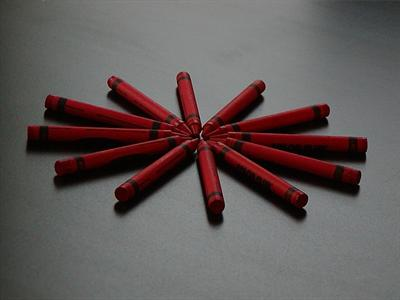
\includegraphics[width=0.45\textwidth]{example1.jpg}} 
  \subfigure[]{ 
    \label{fig: RGBhistogram: b} %% label for second subfigure 
    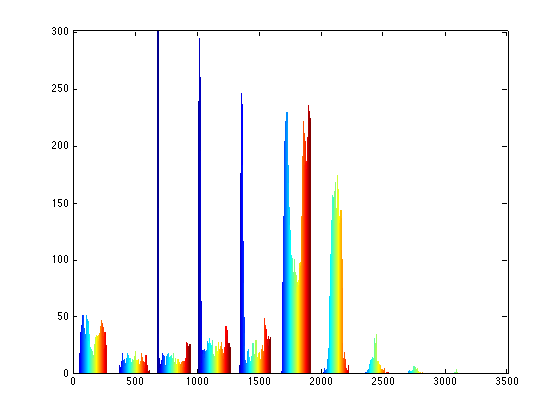
\includegraphics[width=0.45\textwidth]{RGBhistogram1.png}} 
  \caption{RGB空间的颜色直方图}
  \label{fig: RGBhistogram} %% label for entire figure 
\end{figure}

对每个超像素区域,可以知道其中像素点的坐标值,能求出其对应到矩阵$Q$中的值,有多少个不同值就代表该区域内有多少种不同的颜色,然后算该区域在$1-16^3$之间的颜色占的像素个数,没有的记为0。对每个区域都能算出这样一个$16^3$维的向量,然后求区域之间的直方图的对比度,也就是求这样两个向量之间的距离。

PISA~\cite{shi2013pisa}中没有将图像先分割成超像素,求超像素区域间的对比度,但也不是逐像素地计算color contrast。对每个像素点$p$,采用CLMF方法~\cite{lu2012cross}构造一个shape-adaptive observation region $\Omega_p$(如图~\ref{fig: PISA示例}),然后用该区域内的所有像素点$q \in \Omega_p$计算颜色直方图$h^c(p)$。这里用到的是Lab颜色空间,对每个颜色通道量化至12 bins,得到的像素点$p$上的颜色直方图$\mathbf{h}^c(p)$则是一个36维的描述子,如图~\ref{fig: PISA示例}。

\begin{figure}[!ht]
\centering
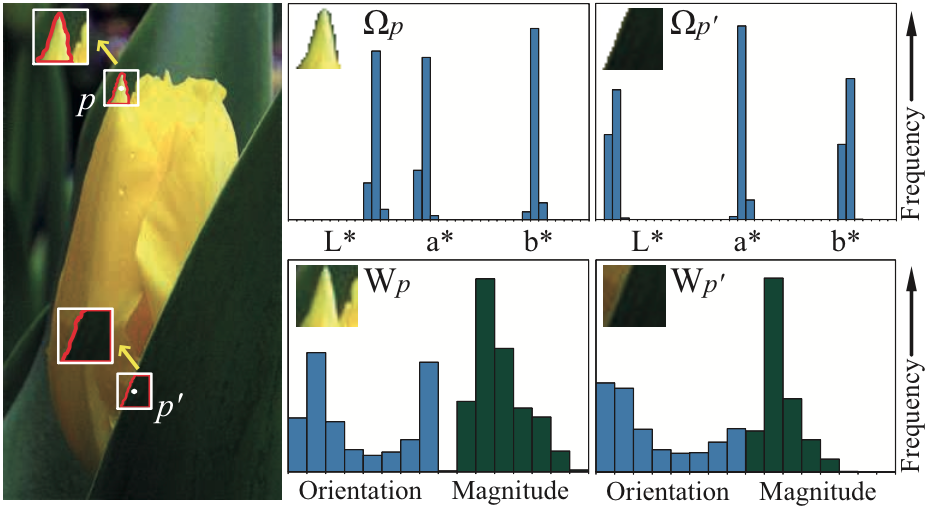
\includegraphics[width=0.6\textwidth]{PISA示例}
\caption{PISA示例}
\label{fig: PISA示例}
\end{figure} 

接着,用k-均值方法将拥有相似颜色直方图的像素聚类到一起。对整幅图像$I$,其颜色特征空间被量化为$K_c$个聚类$\{\Phi_1,\ldots,\Phi_{K_c}\}$。像素上的rarity或contrast计算就可以用聚类间的rarity来近似。假设像素点$p$属于聚类$\Phi_i$,则该点的颜色对比度定义如下:
\begin{align}
U^c(p) = U^c(\mathbf{h}^c(p)) = \sum_{j=1}^{K_c }w_j||\mathbf{h}^c(\Phi_i), \mathbf{h}^c(\Phi_j)||
\end{align}
其中$w_j$表示属于聚类$\Phi_j$的像素个数,$\mathbf{h}^c(\Phi_i)$表示聚类$\Phi_i$内的颜色直方图的均值。

\subsection{纹理特征}

图像纹理一直到现在都没有一个一致的、公认的定义,它在图像中是一个重要但是又不太容易描述出来的特征。纹理是人们将人类的视觉与触觉联系起来,进而形成一个视觉信息,它起源于人类对事物的触感。

LBP(Local Binary Pattern,局部二值模式)首先是由Ojala等人~\cite{ojala1994performance}于1994年提出,DRFI方法~\cite{jianghuaizu2013salient}中用到。

LBP有很多变种,或说改进。原始的LBP记录像素点与其周围像素点的对比信息,或说差异。对于图像上9个方格中中间方格(方格中的值是像素点灰度值大小),做一个阈值化处理。大于等于中心点像素的,标记为1,小于的则标记为0。最后将中心像素点周围的11110001二进制数化为十进制数,得到LBP值。如图~\ref{fig: LBP}所示。

\begin{figure}[!ht]
\centering
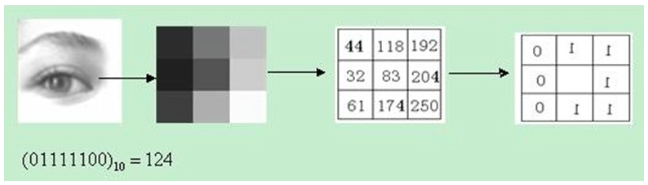
\includegraphics[width=0.6\textwidth]{LBP.png}
\caption{原始LBP}
\label{fig: LBP}
\end{figure} 

实验效果如图~\ref{fig: LBP特征}。

\begin{figure}
  \centering 
  \subfigure[]{ 
    \label{fig: LBP: a} %% label for first subfigure 
    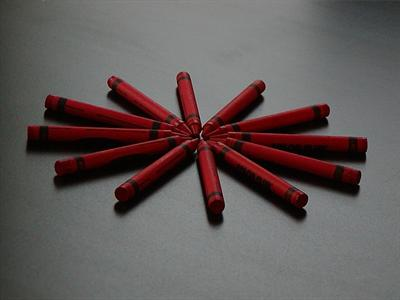
\includegraphics[width=0.45\textwidth]{example1.jpg}} 
  \subfigure[]{ 
    \label{fig: LBP: b} %% label for second subfigure 
    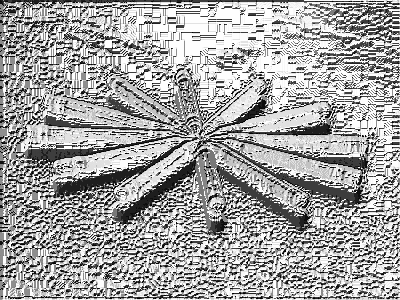
\includegraphics[width=0.45\textwidth]{LBP1.png}} 
  \caption{LBP}
  \label{fig: LBP特征} %% label for entire figure 
\end{figure}

\subsection{Location Contrast}

超像素区域中心与图像中心的距离。每个区域的location contrast只与图像中心有关,而与其它区域没有关系。

论文~\cite{yan2013hierarchical}中用到,公式如下:
\begin{align}
H_i = \frac{1}{w(R_i)}\sum_{x_i \in R_i} exp\{-\lambda||x_i-x_c||^2\}
\end{align}

其中$(x_0, x_1 \ldots)$是区域$R_i$中的像素坐标集,$x_c$是图像中心的坐标,$w(R_i)$计算了区域$R_i$内的像素个数。由$H_i$的公式可看到,距离图像中心越近的区域拥有越大的权值。

\subsection{奇异值特征}

1、HDCT~\cite{kim2014salient}中用到。奇异值特征(Singular Value Feature,SVF)~\cite{su2011blurred}被用来从测试图像中检测模糊区域,通常一幅图像中的模糊区域是背景的可能性较大。

\subsection{HOG特征}

HDCT~\cite{kim2014salient}中用到。HOG(Histogram of Oriented Gradients,方向梯度直方图)特征最早是由法国国家计算机技术和控制研究所(INRIA)的Navneet Dalal和Bill Triggs在2005年发表在CVPR上的论文~\cite{dalal2005histograms}中提出的。

Dalal提出的HOG特征提取的过程如图~\ref{fig: HOG},进一步表述如下:

\begin{figure}[!ht]
\centering
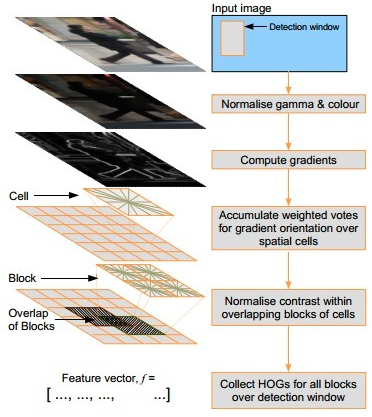
\includegraphics[width=0.6\textwidth]{HOG.png}
\caption{算法流程图}
\label{fig: HOG}
\end{figure} 

1)灰度化

2)采用Gamma校正法对输入图像进行颜色空间的标准化(归一化);目的是调节图像的对比度,降低图像局部的阴影和光照变化所造成的影响,同时可以抑制噪音的干扰。Gamma压缩公式:
\begin{align}
I(x, y) = I(x, y)^{gamma}
\end{align}

3)计算图像每个像素的梯度(包括大小和方向),主要是为了捕获轮廓信息,同时进一步弱化光照的干扰。

图像中像素点$(x, y)$的梯度为
\begin{align}
G_x(x, y) = H(x+1, y) - H(x-1, y) \\
G_y(x, y) = H(x, y+1) - H(x, y-1)
\end{align}

式中$G_x(x, y), G_y(x, y), H(x, y)$分别表示输入图像中像素点$(x, y)$处的水平方向梯度、垂直方向梯度和灰度值。像素点$(x, y)$处的梯度幅值和梯度方向分别为:
\begin{align}
G(x, y) & = \sqrt{G_x(x, y)^2 + G_y(x, y)^2}\\
\alpha(x, y) & = tan^{-1}(\frac{G_y(x, y)}{G_x(x, y)}
\end{align}

最常用的方法是:首先用$[-1, 0, 1]$梯度算子对原图像做卷积运算,得到$x$方向(水平方向,以向右为正方向)的梯度分量gradscalx,然后用$[1, 0, -1]^T$梯度算子对原图像做卷积运算,得到$y$方向(竖直方向,以向上为正方向)的梯度分量gradscaly。然后再用以上公式计算该像素点的梯度大小和方向。

4)将图像每$16*16$(取其它也可以)个像素分到一个cell中,对于$256*256$的图像来说,就分成了$16*16$个cell了。

5)对于每个cell求其梯度方向直方图,通常取$bin = 9$(取其它也可以)个方向(特征),也就是每$360/9 = 40$度分到一个方向,形成每个cell的descriptor。如图~\ref{fig: 方向梯度},当某像素的梯度方向是20-40度,然后它的梯度大小是$|grad|$,那么直方图第2
个bin的计数就要加上$|grad|$。

\begin{figure}[!ht]
\centering
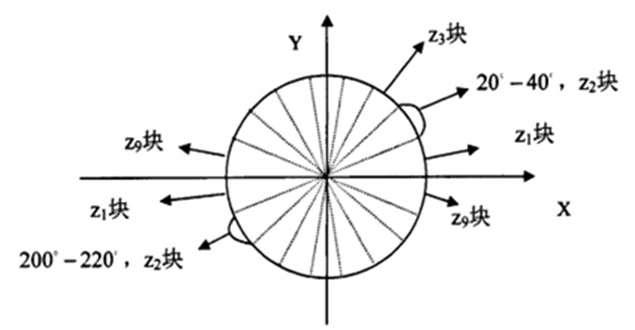
\includegraphics[width=0.5\textwidth]{方向梯度.png}
\caption{梯度方向bin的划分}
\label{fig: 方向梯度}
\end{figure} 

6)由于局部光照的变化以及前景-背景对比度的变化,使得梯度强度的变化范围非常大。这就需要对梯度强度做归一化。归一化能够进一步地对光照、阴影和边缘进行压缩。为此可以将每$2*2$(取其它也可以)个cell合成一个大的、空间上连通的block,所以这里就有$(16-1)*(16-1) = 225$个block。一个block内所有cell的特征向量串联起来便得到该block的HOG特征。这些block是互有重叠的,这就意味着:每一个cell的特征会以不同的结果多次出现在最后的特征向量中。

7)所以每个block中都有$2*2*9$个特征,一共有225个block,所以总的特征有$225*36$个。

遇到的疑问:

1)在显著性检测中,先将图像分割成区域,然后怎么提取该区域的HOG特征?

2)一定要将彩色图像先转化为灰度图像才能提取HOG特征吗?

HDCT~\cite{kim2014salient}方法中用到HOG特征~\cite{felzenszwalb2010object},采用的是VLFeat官网上的代码。论文中首先也是对图像进行超像素分割,然后求每个超像素区域内像素点坐标的平均值$(x_i, y_i)$,$i$代表第$i$个超像素区域,求该区域的HOG特征就是以该坐标点为中心的$17*17$的网格作为输入图像(只取该网格内图像r通道的值),17作为cellSize,然后对每个超像素区域得到一个31维的HOG特征向量。

2、PISA~\cite{shi2013pisa}中用到Structure-Based Contrast。这种结构描述子是对像素点$p$周围的矩形区域$W_p$内的梯度分布用直方图$h^g(p)$来建模。$h^g(p)$计算了包含梯度方向分量和幅值分量的向量出现的频率。论文中将每个分量量化为8个bins,并且称得到的特征空间为OM空间(16维)。$W_p$窗口被固定为$9 \times 9$,最终求出的描述子被称为OM结构描述子。

计算完每个像素上的结构描述子后,用k-均值方法将OM特征空间分成$K_g$个聚类$\{\varphi_1,\ldots,\varphi_{K_g}\}$。计算像素点$p$上的结构对比度等价于计算$p$所属聚类$\varphi_i$上的对比度
\begin{align}
U^g(p) = U^g(\textbf{h}^g(p)) = \sum_{j=1}^{K_g} w_j||\textbf{h}^g(\varphi_i), \textbf{h}^g(\varphi_j)||
\end{align}
$w_j$是聚类$\varphi_j$中像素的个数,$\textbf{h}^g(\varphi_i)$是聚类$\varphi_i$中的OM直方图的均值。

\subsection{Visual Complexity Contrast}

论文~\cite{zhu2014tag}中用到,信息论中可以用熵来计算visual complexity,区域$r_i$和$r_j$之间的visual complexity contrast $D_e(r_i, r_j)$就被定义为
\begin{align}
D_e(r_i, r_j) = [H(r_i)-H(r_j)]^2
\end{align}
其中,$H(r_i)$表示区域$r_i$内的熵
\begin{align}
H(r_i) = \sum_{p=1}^{n_{c, i}}f(c_{p, i})\cdot log_2f(c_{p, i})
\end{align}
其中,$c_{p, i}$是区域$r_i$中第$p$种颜色,$n_{c, i}$区域$r_i$中包含的颜色个数,$f(c_{p, i})$表示区域$r_i$中颜色$c_{p, i}$出现的概率。

\subsection{Background Weighted Contrast}

RBD~\cite{zhu2014saliency}中用到,其中将background weighted contrast定义为
\begin{align}
wCtr(p) = \sum_{i=1}^{N}d_{app}(p, p_i)w_{spa}(p, p_i)w_i^{bg},
\end{align}

\section{Regional property descriptor}

区域性质描述子中涉及的特征是从各区域独立提取的,区域之间相互没有关系,即不存在区域对比度。

\subsection{几何特征}

几何特征一般包括了大小和位置信息,用来描述显著物体和背景的空间分布。例如,显著物体通常位于靠近图像中心的位置,而背景通常分散在整幅图像上。

1、区域内像素点$x$坐标/$y$坐标的平均值

2、整个区域内像素的$x$坐标的$10\%$和$90\%$、$y$坐标的$10\%$和$90\%$

 3、区域周长
 
 4、由2所形成的bounding box的长宽比
 
 5、区域面积
 
 6、性质相近的邻域的面积
 
 \subsection{外观特征}
 
 外观特征通常用来描述区域内的颜色和纹理分布,这样可以描述出显著物体或背景的共同特征,例如,背景通常具有均匀的颜色分布和相似的纹理图案。

1、颜色分布

区域内像素点上RGB值的方差(3维)、L*a*b*值的方差(3维)、HSV值的方差(3维)

2、纹理分布

LM滤波结果的方差

\section{Hierarchical over-segmentation}

方法TS~\cite{zhu2014tag}中用到,hierarchical over-segmentation是通过先对原图像进行超像素分割,再通过迭代将每一分割层再分割成更精细的子区域来实现。

论文~\cite{yan2013hierarchical}中对原图像先提取3个layers,即对原图像($400 \times 300$)用watershed-like方法~\cite{gonzalez2009digital}进行初始的过分割,对每个分割区域计算一个scale值,然后对所有区域的scale值按从小到大排序,如果一个区域的scale值小于3,就将它和最近的区域合并(通过判断两个区域内CIELUV颜色均值的距离),然后更新它的scale,并更新合并区域的颜色均值,等对所有区域都处理后,得到的结果就是$L^1$层。$L^2$层是通过对$L^1$层采取同样的步骤,只不过用一个更大的阈值17。$L^3$层也是如此,阈值取33。

\section{Priors}

\subsection{Center Prior或Location Prior}

SDSP~\cite{zhang2013sdsp}中将Location Prior描述为:处于图像偏中央位置的物体更能吸引人的注意。这里Location Prior是按像素级计算的,定义如下:
\begin{align}
S_D(x) = exp\left(-\frac{||x-c||_2^2}{\sigma_D^2}\right)
\end{align}
效果如图~\ref{fig: SDSPCenterPrior}。
\begin{figure}[!ht]
\centering

\includegraphics[width=0.25\textwidth]{SDSPCenterPrior.png}
\caption{SDSP: Center Prior}
\label{fig: SDSPCenterPrior}
\end{figure} 

PBS~\cite{yang2013graph}中用到Convex-Hull-Based Center Prior,即首先估计显著目标的中心位置$(x_0, y_0)$,再计算每个超像素$i$的显著性:
\begin{align}
S_{ce}(i) = exp\left(-\frac{||x_i-x_0||^2}{2\sigma_x^2}-\frac{||y_i-y_0||^2}{2\sigma_y^2}\right)
\end{align}

\subsection{Backgroundness Prior}

通常是基于伪背景的假设,即假设处于图像周围狭窄边界上的区域是背景区域。

1、2012年,论文~\cite{wei2012geodesic}中提出了关于background的两种prior,叫做boundary and connectivity priors。boundary prior来源于摄影构图的基本规则,大部分摄影师都不会将显著目标切断在视觉框架中,也就是说,位于图像边界上的通常是背景。这个prior比之前提出的center prior更通用一些,因为显著目标可能并不会正好位于图像正中央,例如三分构图法,但它们很少会处在图像边界上。connectivity prior是从图像中背景的外观特征得来的,背景区域通常较大并且是同质的。也就是说,背景中绝大多数图像块可以很容易地彼此连接起来。如图~\ref{fig: GS}。
\begin{figure}[!ht]
\centering
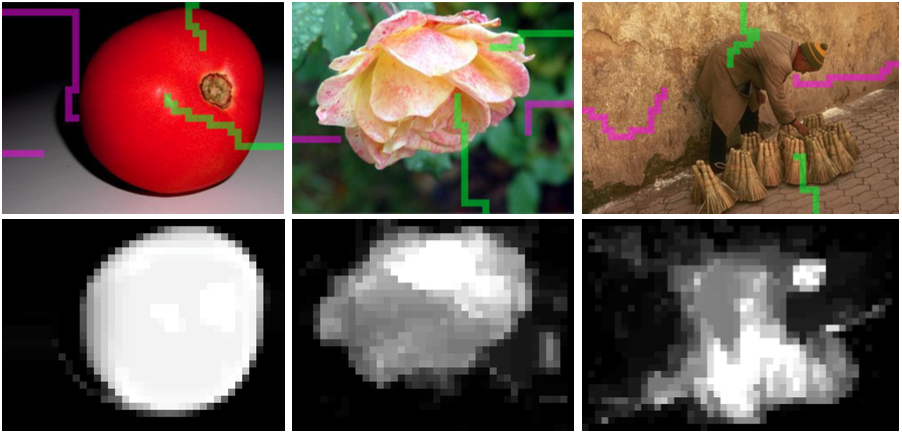
\includegraphics[width=0.5\textwidth]{GS.png}
\caption{Geodesic saliency图例}
\label{fig: GS}
\end{figure} 

首先対一幅图像构造无向图$G = \{V, \varepsilon \}$,图中的节点由两部分(图像块$\{P_i\}$和伪背景节点$B$)构成,即$V = \{P_i\}\cup \{B\}$。边也包括两种类型,一种是internal edges,连接了所有相邻的图像块,另一种是boundary edges,连接了处于图像边界的块和背景节点,即$\varepsilon = \{(P_i, P_j)|$$P_i$与$P_j$相邻$\} \cup \{(P_i, B)|$$P_i$在图像边界上\}。

图像块$P$上的geodesic saliency被定义为沿着从$P$到背景节点$B$的最短路径上的边的权值的累加和。
\begin{align}
saliency(P) = \min_{P_1=P, P_2, \ldots, P_n=B}\sum_{i=1}^{n-1}weight(P_i, P_{i+1}), s.t.(P_i, P_{i+1})\in \varepsilon
\end{align}

1)伪背景的节点是怎么找的?

2)如何求internal edge weight?

internal edge weight是相邻图像块之间的appearance distance,采用的是一种简单有效的weight clipping approach,图像块与块之间的appearance distance求的是两个块在LAB颜色空间上的颜色平均值的不同。对图像中的每一个块,算出它与所有neighbors的最小appearance distance,然后取这些distance的均值作为“insignificance” distance threshold,当某距离比这个阈值小时就说明它是不重要的,将它置为0。

3)如何求boundary edge weight?

boundary edge weight度量的是处于图像边界的图像块不是背景的可能性大小。当boundary prior是完全有效的时候,所有的boundary edge weight就都是0。但现实没有这么理想化,显著目标只要有哪怕一小部分落到了图像边界,也会产生不好的效果。这里可以通过用其他的显著性的方法来实现,已知图像边界上的块,计算每个块$P_i$的显著性作为the weight of boundary edge($P_i, B$)。

MR~\cite{yang2013saliency}算法步骤如图~\ref{fig: MR1},先对图像进行超像素分割,然后将分割后的图像映射为图,每个超像素为图中的节点。第一个阶段是将图像的每一条边界上(共4条)的节点看作是labelled background queries,依次算图中的每个节点与这些queries的相关性来得到4幅labelled maps,然后对其进行融合得到显著图。在第二阶段,对第一阶段得到的显著图二值化,然后将得到的labelled foreground节点看作是salient queries,最终每个节点的显著度就是通过计算其与foreground queries的相关性得到。
\begin{figure}[!ht]
\centering
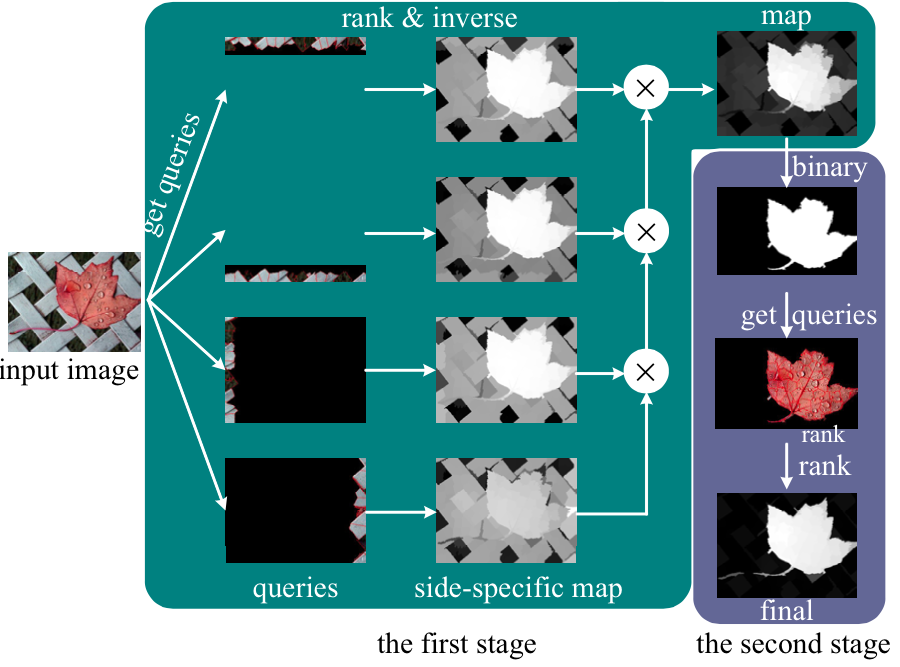
\includegraphics[width=0.7\textwidth]{MR1.png}
\caption{算法步骤}
\label{fig: MR1}
\end{figure}

2、论文~\cite{jiang2013saliency}中也用到backgroundness prior,即将图像四周边界看成是伪背景节点,将马尔可夫随机游走的性质与显著性检测联系起来。

3、OptSeedProp~\cite{lu2014learning}中用到

\subsection{Boundary connectivity prior}

由于基于伪背景假设的显著目标检测方法在目标碰到图像边界时会失效,所以后来又提出了boundary connectivity prior,这种prior被描述为:显著目标与图像边缘的连接程度比背景与边缘的连接程度小。

论文~\cite{zhu2014saliency}中将一个区域内的boundary connectivity score定义为它沿图像边缘的长度与整个区域面积的比值:
\begin{align}
BndCon(p) = \frac{Len_{bnd}(p)}{\sqrt{Area(p)}}
\end{align}

\subsection{Color Prior}

SDSP~\cite{zhang2013sdsp}中将Color Prior描述为:暖色(例如红色和黄色)比冷色(例如绿色和蓝色)更能吸引人类视觉系统的注意。先将图像由RGB颜色空间转换到$CIEL*a*b*$空间,$\{ f_L(x)\}$, $\{ f_a(x)\}$, $\{ f_b(x)\}$分别代表$L*$通道,$a*$通道和$b*$通道。这里Color Prior是按像素级计算的,定义如下:
\begin{align}
S_c(x) = 1-exp\left(-\frac{f_{an}^2(x)+f_{bn}^2(x)}{\sigma_c^2}\right)
\end{align}
其中
\begin{align}
f_{an}(x)=\frac{f_a(x)-mina}{maxa-mina}, f_{bn}(x) = \frac{f_b(x)-minb}{maxb-minb}
\end{align}
效果如图~\ref{fig: SDSPColorPrior}。
\begin{figure}
  \centering 
  \subfigure[]{ 
    \label{fig: SDSPColorPrior: a} %% label for first subfigure 
    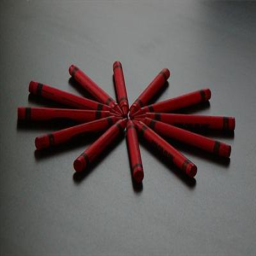
\includegraphics[width=0.25\textwidth]{example2.png}} 
  \subfigure[]{ 
    \label{fig: SDSPColorPrior: b} %% label for second subfigure 
    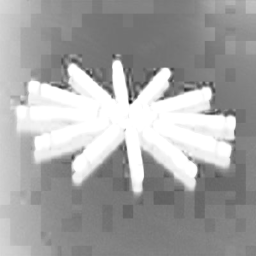
\includegraphics[width=0.25\textwidth]{SDSPColorPrior.png}} 
  \caption{SDSP: Color Prior}
  \label{fig: SDSPColorPrior} %% label for entire figure 
\end{figure}

\subsection{Objectness Prior}

论文~\cite{chang2011fusing}中将objectness与regional saliency融合,形成一个graphical model。

论文~\cite{jiangpeng2013salient}中从两个方面估计objectness,一是pixel-level objectness estimation,二是region-level objectness estimation。

Pixel-level Objectness:每个像素点的objectness值是以该像素点为中心的局部窗口内包含完整目标的概率。在图像上随机抽样$N$个窗口,求每一个窗口$w$上用来表示objectness的概率值$P(w)$。将所有窗口集记作$W$,对每个像素点$x$可以得到它的像素级objectness $O_p(x)$
\begin{align}
O_p(x) = \sum_{w \in W \text{ }and \text{ } x \in w} P(W_x),
\end{align}
$w$表示$W$中包含像素点$x$的任意窗口,论文中取$N=10000$。

Region-level Objectness:对每个区域$\Lambda_i$,计算该区域内的region-level objectness $O_r(\Lambda_i)$为:
\begin{align}
O_r(\Lambda_i) = \frac{1}{|\Lambda_i|}\sum_{x \in \Lambda_i} O_p(x).
\end{align}
计算完一个区域内的objectness后,把这个值赋给该区域内的所有像素。这样就可以得到整幅图像I的objectness map,简称为$O(I)$。

\subsection{Smoothness Prior}

PBS~\cite{yang2013graph}中用到,平滑约束通常是用在基于图的目标分割中,目的是使图像中相邻的像素拥有同样的label值。论文中先将图像分割成超像素,然后将其映射为图,每个超像素对应图中的节点,有共同的边界的超像素之间有一条边,边上的权值为$w_{ij} \in W$:
\begin{align}
w_{ij} = exp\left(-\frac{||c_i-c_j||}{2\sigma_w^2}\right),
\end{align}
其中$c_i$和$c_j$是CIELab空间超像素区域内像素的颜色均值。可以看到关系矩阵$W$是一个稀疏矩阵。定义如下saliency cost function来表示这种smoothness prior:
\begin{align}
E(S) = \sum_i(S(i)-S_{in}(i))^2+\lambda\sum_{i,j}w_{ij}(S(i)-S(j))^2
\end{align}
$S(i)$和$S(i)$分别表示节点$i$和$j$的所要求的显著值,$S_{in}(i)$是节点$i$的初始显著值,$\lambda$是规范化系数。其中等式右边第一项是fitting constraint,表示一幅好的显著图与初始显著图之间不会变化太多。第二项是smoothness constraint,一幅好的显著图上相邻超像素的显著值不会相差太多。超像素上的最优显著值是通过最小化该cost function来计算。令该方程关于$S$的导数为0可得
\begin{align}
S^* = \mu (D-W+\mu I)^{-1}S_{in}
\end{align}
其中$D$是三角矩阵,并且有$d_{ii} = \sum_j (w_{ij})$,$\mu = 1/(2\lambda)$。

\subsection{Focusness Prior}

论文~\cite{jiangpeng2013salient}中将focusness定义为焦点模糊程度。

\section{Feature Contrasts/Priors的融合}

\subsection{相乘}

对相乘融合而言,要保证相乘的量取值在$[0, 1]$之间。

目前来看,分为两种。

1. 求出两个区域间关于多种关于visual cues的对比度之后,要先将这些对比度融合,例如可以相乘,求出最终的对比度公式。然后再对每个区域计算local或global contrast。

论文~\cite{zhu2014tag}中,两个区域$r_i$、$r_j$间的最终的对比度定义如下:
\begin{align}
D_r(r_i, r_j) = D_c(r_i, r_j) \cdot exp[\sigma_e^2 \cdot D_e(r_i, r_j)]
\end{align}
其中$D_c(r_i, r_j)$是指color contrast,$D_c(r_i, r_j)$是指visual complexity contrast。

对每个区域$r_i$,其空间加权global contrast定义为:
\begin{align}
U(r_i) = \sum_{j\ne i}w_{ij} \cdot D_r(r_i, r_j) \cdot \phi_j\\
w_{ij} = \frac{1}{Z_i}\cdot exp[-\sigma_s^2 \cdot D_s(r_i, r_j)]
\end{align}
其中,$\phi_j$是指区域$r_j$内的像素个数,即区域$r_j$的大小。$D_s(r_i, r_j)$表示区域$r_i$和$r_j$之间的空间距离。$\phi_s$则用来控制空间加权$w_{ij}$的影响程度,$\phi_s$越大,对$U(r_i)$的影响越小。$\frac{1}{Z_i}$是归一化因子,保证$\sum_{j \ne i}w_{ij} = 1$。

2. 对每个visual cue求出local或global contrast之后,再对这些对比度进行融合。

例如论文~\cite{yan2013hierarchical}中,作者用了两种cues:

1)local contrast

\begin{align}
C_i = \sum_{j=1}^{n}w(R_i)\Phi(i, j)||c_i-c_j||_2
\end{align}
其中$c_i$和$c_j$分别表示区域$R_i$和$R_j$中的颜色,$w(R_j)$指$R_j$中像素的个数。$\Phi(i, j) = exp\{-D(R_i, R_j)/\sigma^2\}$,控制了区域$R_i$和$R_j$之间的空间距离,其中$D(R_i, R_j)$是区域$R_i$和$R_j$的中心的欧几里得距离的平方。

2)location heuristic

心理物理学方面的研究表示人类视觉注意偏好图像的中央区域,所以在通常情况下越靠近图像中央的像素越显著。
\begin{align}
H_i = \frac{1}{w(R_i)}\sum_{x_i \in R_i} exp\{-\lambda||x_i-x_c||^2\}
\end{align}
其中$\{x_0, x_1\ldots\}$是区域$R_i$中的像素坐标的集合,$x_c$是图像中心坐标。

然后将$C_i$与$H_i$组合起来,得到
\begin{align}
\bar{s}_i = C_i \cdot H_i
\end{align}

方法PBS~\cite{yang2013graph}中在求初始显著图时先计算了spatially weighted contrast
\begin{align}
S_{co}(i) = \sum_{j \ne i}||c_i-c_j|| \cdot exp\left(-\frac{||p_i-p_j||^2}{2\sigma_p^2}\right)
\end{align}
然后又计算了convex-hull-based center prior map,即首先估计显著目标的中心位置$(x_0, y_0)$,再计算每个超像素$i$的显著性:
\begin{align}
S_{ce}(i) = exp\left(-\frac{||x_i-x_0||^2}{2\sigma_x^2}-\frac{||y_i-y_0||^2}{2\sigma_y^2}\right)
\end{align}
最后将两者相乘得到初始显著图
\begin{align}
S_{in}(i) = S_{co}(i) \times S_{ce}(i)
\end{align}


\subsection{相加}

\subsection{利用机器学习进行优化}

\subsubsection{基于图的显著性检测方法}

能量方程

1、论文~\cite{zhu2014saliency}中是通过最小二乘实现全局优化。其中的cost function如下:
\begin{align}
\sum_{i=1}^{N}w_i^{bg}s_i^2+\sum_{i=1}^{N}s_i^{fg}(s_i-1)^2+\sum_{i, j}w_{ij}(s_i-s_j)^2,
\end{align}
其中第一项是背景约束,当某区域的$w_i^{bg}$较大时,是背景的概率较大,方程的第一项占的比重较多,为使整个方程值最小,需使$s_i$近似为0,也就是使该区域的显著性近似为0。第二项是前景约束,当某区域的$w_i^{fg}$较大时,第二项占的比重较大,需使$s_i$近似为1。$w_i^{fg}$可以通过目前已有的一些显著性方法或它们的组合来计算。第三项是平滑约束,保证显著值的连续性,$w_{ij}$定义如下:
\begin{align}
w_{ij} = exp(-\frac{d_{app}^2(p_i, p_j)}{2\sigma_{clr}^2})+\mu
\end{align}
超像素$p_i$与$p_j$越相似,$d_{app}(p_i, p_j)$越小,$w_{ij} $越大,越需要$s_i$,$s_j$近似相等。

2、方法PBS~\cite{yang2013graph}中求最终显著图时用到如下saliency cost function:
\begin{align}
E(S) = \sum_i(S(i)-S_{in}(i))^2+\lambda\sum_{i,j}w_{ij}(S(i)-S(j))^2
\end{align}
$S(i)$和$S(i)$分别表示节点$i$和$j$的所要求的显著值,$S_{in}(i)$是节点$i$的初始显著值,$\lambda$是规范化系数。其中等式右边第一项是fitting constraint,表示一幅好的显著图与初始显著图之间不会变化太多。第二项是smoothness constraint,一幅好的显著图上相邻超像素的显著值不会相差太多。超像素上的最优显著值是通过最小化该cost function来计算。

条件随机场

条件随机场(Conditional Random Fields, CRFs)最早由Lafferty等人~\cite{lafferty2001conditional}于2001年提出,其模型思想主要来源于最大熵模型。


马尔可夫随机场

\section{显著图的融合}

1、论文~\cite{borji2012salient}中是将由图像$I$得到的$m$幅显著图$\{S_i||1 \le i \le m \}$通过如下方式融合得到最终的显著图:
\begin{align}
S(p) = P(y_p=1|S_1(p), S_2(p), \ldots, S_m(p))\propto \frac{1}{Z} \sum_{i=1}^{m} \zeta(S_i(p)), 
\label{align: bayesian}
\end{align}
其中,$S(p)$表示图像$I$上像素点$p$处的显著值,$S_i(p)$表示显著图$S_i$上像素点$p$处的显著值,$y_p$是一个二值随机变量,当像素点$p$是显著的时值为1,否则值为0,$Z$是一个常数。

由方程~(\ref{align: bayesian})可看出,当有一个方法产生的值很小时,在相乘时对整个结果影响较大,论文中对函数$\zeta$采用了三种改进形式,包括:
\begin{align}
\zeta_1(x) = x, \, \zeta_2(x) = exp(x), \,and \, \zeta_3(x) = \frac{-1}{log(x)}
\end{align}
当进行融合的方法的性能之间相差较大时,这种融合方法效果不是很好,主要原因是没有考虑到不同方法的效果差异而将它们同等对待。因此,性能较差的方法会在最终融合效果中占主导作用。

2、论文~\cite{mai2013saliency}中采用了两种显著性融合方法。

第一种(pixel-wise aggregation):对图像中的每个像素点$p$,对应一个特征向量$\textbf{x}(p) = (S_1(p), S_2(p), \ldots, S_m(p))$,其中$S_i(p)$是像素点$p$在显著图$S_i$中的显著值。这里也定义了一个二值的随机变量$y_p$,表征某像素是否是显著的。如果像素点$p$是显著的值就为1,反之值为0。最终的显著值$S(P)$可看成是求取后验概率$P(y_p = 1|x(p))$,这个后验概率可以用logistic model~\cite{bishop2006pattern}来建模,
\begin{align}
P(y_p=1|x(p);\lambda)=\sigma(\sum_{i=1..m}\lambda_i S_i(p)+\lambda_{m+1})
\end{align}
其中模型参数$\lambda = \{\lambda_i|i=1..m+1\}$权衡了每幅显著图的贡献大小。这里$\sigma(.)$指的是如下的sigmoid函数
\begin{align}
\sigma(z) = \frac{1}{1+exp(-z)}
\end{align}
参数$\lambda$可以通过在训练集上用standard logistic regression technique学习到。

第二种(CRF-based aggregation):第一种方法分别计算各个像素上的显著值,而忽略了相邻像素间的关系。第二种方法有效解决了该问题,通过二值条件随机场~\cite{lafferty2001conditional}来估计显著值。利用条件随机场可以获取相邻像素间的相互关系。

像第一种方法一样,将每个像素看成是一个节点,对应每个节点有一个特征向量$\textbf{x}(p) = (S_1(p), S_2(p), \ldots, S_m(p))$和一个二值随机标签$y_p$,1代表显著的,0代表非显著的。每个像素点上的显著性标签不仅依赖于它的特征向量,还依赖于相邻像素点上的标签。像素之间的相互关系也依赖于其上的特征。论文中使用网格形状的条件随机场来对标签和特征间的关系、相邻像素间标签的特征依赖关系进行建模。定义特征$X=\{x_p|p\in I\}$上的标签$Y=\{y_p|p \in I\}$的条件分布如下:
\begin{align}
P(Y|X;\theta) = \frac{1}{Z}exp(\sum_{p\in I}f_d(\textbf{x}_p, y_p)+\sum_{p \in I}\sum_{q\in N_p}f_s(\textbf{x}_p, \textbf{x}_q, y_p, y_q))
\end{align}
其中$p$是图像$I$中的一个像素,$\textbf{x}_p$表示其上的特征,$y_p$是它的显著性标签,$\theta$是条件随机场模型的参数。$f_d(\textbf{x}_p, y_p)$是定义特征和标签之间关系的特征函数。$f_s(\textbf{x}_p, \textbf{x}_q, y_p, y_q)$是另一个定义相邻像素$p$和$q$标签的特征依赖关系的特征函数。$N_p$是与$p$相关的像素集合。这里表示8邻域关系。$Z$是一个常数。

特征函数$f_d(\textbf{x}_p, y_p)$的定义仅仅与输入的显著图$S_i$有关,
\begin{align}
f_d(\textbf{x}_p, y_p) = \sum_{i=1}^{m}\lambda_iS_i(p)y_p+\lambda_{m+1}y_p
\end{align}
其中$\{\lambda_i\}$是条件随机场模型的参数集,$S_i(p)$是显著图$S_i$中像素点$p$处的显著值。

特征函数$f_s(\textbf{x}_p, \textbf{x}_q, y_p, y_q)$由两个分量组成,
\begin{align}
f_s(\textbf{x}_p, \textbf{x}_q, y_p, y_q) = f_e(\textbf{x}_p, \textbf{x}_q, y_p, y_q)+f_c(\textbf{x}_p, \textbf{x}_q, y_p, y_q)
\end{align}
第一个分量$f_e(\textbf{x}_p, \textbf{x}_q, y_p, y_q)$表示如果两个像素点用同一种显著性方法计算出的显著值不同,它们在融合结果中就可能会有不同的显著性标签。
\begin{align}
f_e(\textbf{x}_p, \textbf{x}_q, y_p, y_q) = \sum_{i=1}^{m}\alpha_i(\textbf{1}(y_p=1, y_q=0)-\textbf{1}(y_p=0, y_q=1))(S_i(p)-S_i(q))
\end{align}
其中,$\alpha$是这个特征函数中条件随机场模型的参数,$\textbf{1}(.)$是一个indicator函数。

$f_c(\textbf{x}_p, \textbf{x}_q, y_p, y_q)$与论文~\cite{liu2011learning}中思路一样,表示有相似颜色的相邻像素应该有相似的显著性标签。
\begin{align}
f_c(\textbf{x}_p, \textbf{x}_q, y_p, y_q) = -\textbf{1}(y_p\ne y_q)exp(-\eta||I(p)-I(q)||)
\end{align}
其中,$||I(p)-I(q)||$是RGB颜色空间中像素$p$和$q$之间的差异。$\eta$




%
% references
\bibliographystyle{plain}

\bibliography{FeaturesPriors} %参考文献


\end{document}